\documentclass[11pt]{article}

\usepackage[margin=1in]{geometry}
\usepackage[T1]{fontenc}
\usepackage[utf8]{inputenc}
\usepackage{lmodern}
\usepackage{amsmath}
\usepackage{amssymb}
\usepackage{booktabs}
\usepackage{enumitem}
\usepackage{hyperref}
\usepackage{graphicx}
\usepackage{xcolor}
\usepackage{tikz}
\usetikzlibrary{arrows.meta,positioning,calc}

\hypersetup{
  colorlinks=true,
  linkcolor=blue!60!black,
  urlcolor=blue!60!black,
  citecolor=blue!60!black
}

\setlist[itemize]{leftmargin=1.5em}
\setlength{\parskip}{0.5em}
\setlength{\parindent}{0pt}

\title{Hybrid Quantum Time-Series Forecasting for Wildfire Risk and Insurance Modeling}
\author{%
  Tawheed Islam Bhuian and Dhanush Kankanala \\
  Team: BU-Quantum \\
  State University of New York at Binghamton \\
  Binghamton, NY, USA \\
  \texttt{\{mislambhuian, dkankanala\}@binghamton.edu} \\
}
\date{}
\begin{document}
\maketitle

\begin{abstract}
This submission presents a hybrid quantum--classical machine learning pipeline for wildfire-risk forecasting and downstream insurance-premium modeling at the California ZIP-code level. The solution builds on two state-of-the-art multivariate time-series forecasting backbones---FreTS and Crossformer---and augments them with shallow variational quantum circuits (VQCs) implemented in PennyLane. Rather than appending a quantum post-processing layer to the model output, the proposed deep hybrid variants, \texttt{QFreTS\_Deep} and \texttt{QCrossformer\_Deep}, inject quantum computation into internal feature-processing stages where cross-variable interactions and latent compression are most critical.

The hybrid pipeline operates on complete 2018--2021 ZIP/year panels, using the 2018--2020 history as input and predicting the 2021 wildfire-risk target. Each quantum insertion point maps classical features into a low-qubit latent space via a shared \emph{Quantum Residual Block}, applies angle embedding and trainable variational rotations with entangling gates, and returns Pauli-$Z$ expectation values that are fused back into the classical network through residual connections and layer normalization.

A comprehensive benchmark evaluates the hybrid models against 25 classical time-series baselines from the Time-Series-Library on both a 9-feature minimal and a 20-feature extended dataset. Evaluation is performed using MAE, MSE, RMSE, and $R^2$ on held-out ZIP codes, with feature normalization fitted strictly on the training split. The primary contribution is architectural: demonstrating that a compact quantum block can be inserted at high-value interaction points of a strong classical forecaster and remain competitive while using only 4 qubits and 1--2 variational layers on a statevector simulator.
\end{abstract}

\newpage

\section{Detailed Description of the Participant's Algorithm}

\subsection{Concept}

The central idea is to treat the variational quantum circuit not as a standalone forecasting model, but as a \emph{structured nonlinear interaction module} embedded within a proven classical backbone. The classical model handles large-scale sequence modeling---temporal pattern extraction, frequency-domain transformations, and multi-scale encoding---while the VQC is deployed at specific architectural bottlenecks where compressed, entangled representations may add value. These bottlenecks include cross-variable routing, channel gating, latent refinement, and encoder-to-decoder transfer.

This approach is motivated by a practical observation: current quantum hardware and simulators cannot efficiently process the full dimensionality of a multivariate time-series forecasting problem. However, at certain internal stages of a deep forecasting model, the representation has already been compressed into a low-dimensional summary (e.g., a per-channel gate vector, a pooled embedding, or a bottleneck latent code). These compressed representations are natural candidates for quantum processing because: (i) they can be mapped onto a small number of qubits without aggressive truncation, (ii) their cross-variable structure may benefit from the entanglement-driven correlations inherent in quantum circuits, and (iii) the classical residual pathways ensure that the model degrades gracefully if the quantum contribution is weak.

The design follows three guiding principles:
\begin{itemize}
  \item \textbf{Low qubit count.} Keep the number of qubits small (4 in the primary experiments) so the method remains executable on a statevector simulator and potentially portable to near-term quantum hardware.
  \item \textbf{Bottleneck placement.} Place quantum layers at internal stages where the model has already distilled the raw time series into a compact representation, rather than at the raw input or final output.
  \item \textbf{Classical residual preservation.} Every quantum insertion point maintains a classical skip connection so that gradient flow is not disrupted and the hybrid model can recover classical-only behavior if the quantum parameters do not contribute.
\end{itemize}

\subsection{General Composition}

The end-to-end workflow comprises four stages:
\begin{enumerate}
  \item \textbf{Data aggregation and preprocessing.} Raw wildfire, insurance, weather, and census fields are joined and aggregated to ZIP-year panels. Each panel represents one California ZIP code observed over four consecutive years (2018--2021). The preprocessing script computes derived features---temperature range, drought proxy, log precipitation, dry-hot indicators, burned acres, socioeconomic indices, and cyclical year encodings---and produces two dataset variants: a 9-feature \emph{minimal} set and a 20-feature \emph{extended} set.
  \item \textbf{Task-specific dataset construction.} For Task~1A, the prediction target is \texttt{avg\_fire\_risk\_score}. Each ZIP's 4-year trajectory is split into a 3-step input history (2018--2020) and a 1-step forecast target (2021). For the envisioned Task~2, the target is \texttt{earned\_premium}, and the dataset is augmented with the Task~1A wildfire-risk prediction as an additional explanatory feature.
  \item \textbf{Hybrid quantum--classical forecasting.} A classical backbone (FreTS or Crossformer) is augmented with quantum residual blocks at selected internal computation points. The resulting deep hybrid model is trained end-to-end using standard gradient-based optimization via PennyLane's differentiable quantum simulation.
  \item \textbf{Task chaining.} The predicted 2021 wildfire-risk score from the best Task~1A model is injected into the insurance-premium dataset as a new feature, enabling a second forecasting model to condition premium predictions on the upstream risk forecast.
\end{enumerate}

Figure~\ref{fig:architecture-overview} gives a high-level view of the proposed hybrid pipeline.

\begin{figure}[ht]
\centering
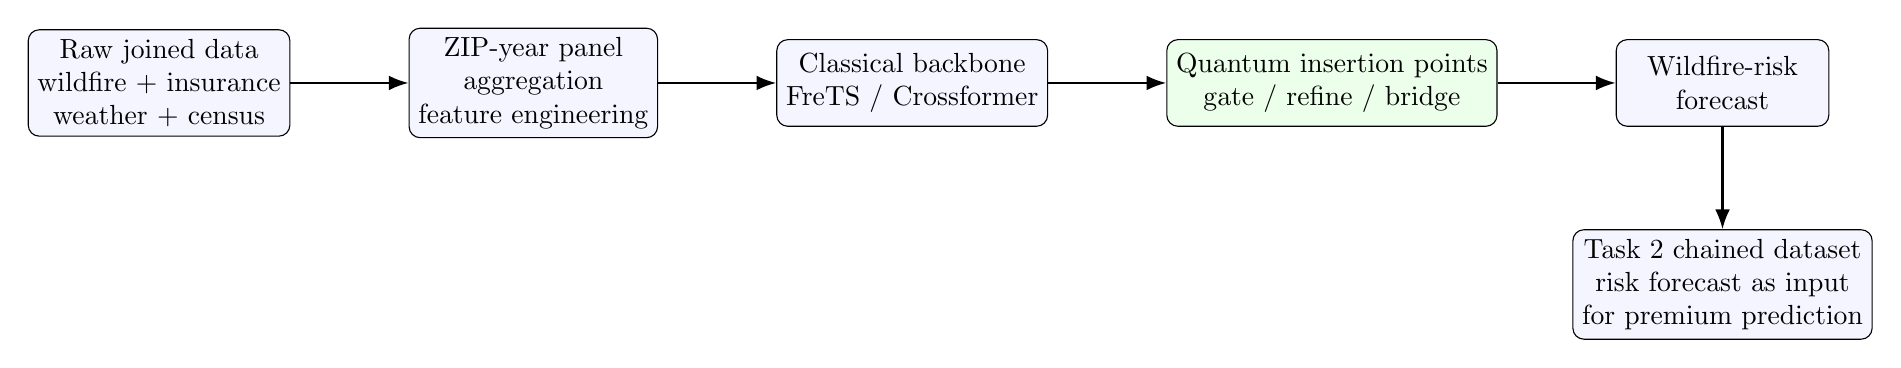
\begin{tikzpicture}[
  node distance=1.5cm,
  box/.style={draw, rounded corners, align=center, minimum height=1.1cm, minimum width=2.7cm, fill=blue!4},
  qbox/.style={draw, rounded corners, align=center, minimum height=1.1cm, minimum width=2.9cm, fill=green!8},
  arr/.style={-{Latex[length=2.5mm]}, thick}
]
\node[box] (data) {Raw joined data\\wildfire + insurance\\weather + census};
\node[box, right=of data] (prep) {ZIP-year panel\\aggregation\\feature engineering};
\node[box, right=of prep] (backbone) {Classical backbone\\FreTS / Crossformer};
\node[qbox, right=of backbone] (quantum) {Quantum insertion points\\gate / refine / bridge};
\node[box, right=of quantum] (forecast) {Wildfire-risk\\forecast};
\node[box, below=1.3cm of forecast] (task2) {Task 2 chained dataset\\risk forecast as input\\for premium prediction};

\draw[arr] (data) -- (prep);
\draw[arr] (prep) -- (backbone);
\draw[arr] (backbone) -- (quantum);
\draw[arr] (quantum) -- (forecast);
\draw[arr] (forecast) -- (task2);
\end{tikzpicture}
\caption{Overview of the hybrid forecasting pipeline from raw data to wildfire-risk prediction and downstream premium modeling.}
\label{fig:architecture-overview}
\end{figure}

\subsection{Classical Baselines}

The hybrid models build directly on two classical backbones from the Time-Series-Library. Understanding these baselines is essential for appreciating where and why quantum computation is inserted.

\subsubsection*{FreTS: Frequency-Domain Time-Series Forecasting}

FreTS operates entirely in the frequency domain. Given an input tensor of shape $[\text{batch}, T, N]$ (where $T$ is the number of time steps and $N$ is the number of variables), FreTS first applies a \emph{token embedding} that projects each scalar value into a $D$-dimensional space via a learned embedding vector, producing a representation of shape $[B, N, T, D]$.

The core computation consists of two frequency-domain MLPs:
\begin{itemize}
  \item \textbf{Channel MLP (\texttt{MLP\_channel}).} The tensor is permuted to $[B, T, N, D]$ and an FFT is applied along the variable dimension $N$. A complex-valued MLP processes the frequency components, mixing information across variables in the spectral domain. An inverse FFT recovers the spatial representation.
  \item \textbf{Temporal MLP (\texttt{MLP\_temporal}).} An FFT is applied along the time dimension $T$, and a second complex-valued MLP processes temporal frequency components. The inverse FFT recovers the time-domain signal.
\end{itemize}

Both MLPs use a \emph{softshrink} activation with a sparsity threshold, promoting sparse frequency-domain representations. After a residual connection from the input embedding, the output is flattened to $[B, N, T \cdot D]$ and passed through a two-layer fully connected prediction head (with LeakyReLU activation and hidden size 256) to produce the final forecast of shape $[B, \text{pred\_len}, N]$.

The key observation for quantum integration is that FreTS processes cross-variable information through the channel MLP in the frequency domain. This stage compresses all $N$ variables into a spectral mixing operation---a natural bottleneck where quantum entanglement could capture higher-order correlations.

\subsubsection*{Crossformer: Cross-Dimension Transformer}

Crossformer is an encoder--decoder Transformer designed specifically for multivariate time series. Its distinguishing feature is the \emph{Two-Stage Attention Layer}, which decomposes attention into cross-time and cross-dimension stages:

\begin{itemize}
  \item \textbf{Patch embedding.} The input time series is segmented into non-overlapping patches of length \texttt{seg\_len}. Each patch is linearly projected to a $d_\text{model}$-dimensional representation, and a learnable positional embedding is added. The resulting tensor has shape $[B, N, S, d_\text{model}]$, where $S$ is the number of segments.
  \item \textbf{Cross-time attention (Stage 1).} For each variable independently, standard multi-head self-attention is applied across the segment axis. This captures temporal dependencies within each variable's trajectory. The attention is followed by LayerNorm and a feedforward MLP.
  \item \textbf{Cross-dimension attention (Stage 2).} The tensor is reshaped so that, for each time segment, all $N$ variables are visible simultaneously. A learned \emph{router} mechanism---consisting of a ``dimension sender'' that projects variables into a shared routing space and a ``dimension receiver'' that reads from it---enables cross-variable information exchange. This router-based design avoids the $O(N^2)$ cost of full cross-variable attention.
  \item \textbf{Multi-scale encoding.} The encoder stacks multiple \texttt{scale\_block} layers, each of which merges adjacent segments (via \texttt{SegMerging}) to capture longer-range dependencies at coarser temporal resolutions.
  \item \textbf{Decoder.} A decoder with cross-attention to the multi-scale encoder outputs produces the final forecast.
\end{itemize}

The cross-dimension routing stage is the architectural bottleneck most amenable to quantum enhancement: it is where all variables interact through a compact intermediate representation, and the router's linear projections could potentially be enriched by quantum entanglement.

\subsection{Quantum Integration: Deep Hybrid Architectures}

Unlike \emph{shallow} quantum wrappers (which simply append a quantum block to the classical model's output), the deep hybrid variants inject quantum circuits at specific internal computation points within the backbone architecture. All quantum insertion points share the same underlying \emph{Quantum Residual Block} (described in Section~\ref{sec:qrb}), but each is applied to a different intermediate representation with different semantic meaning.

\subsubsection*{QFreTS\_Deep}

\texttt{QFreTS\_Deep} modifies the FreTS backbone at three internal stages:

\begin{enumerate}
  \item \textbf{Quantum Channel Gate (replaces \texttt{MLP\_channel}).} Instead of the classical frequency-domain channel MLP, a squeeze-and-excite style gating mechanism is used. The embedded representation $[B, N, T, D]$ is globally averaged across the time and embedding dimensions to produce a per-channel summary $[B, N]$. This summary is processed through a VQC, which sees all $N$ channels simultaneously---the entangling gates create quantum correlations between channel qubits, allowing the gate to capture nonlinear cross-variable dependencies. The VQC output is passed through a sigmoid activation to produce a multiplicative gate $[B, N]$ that modulates each channel's contribution. This requires $B$ circuit evaluations per forward pass.

  \item \textbf{Quantum Embedding Refinement (new stage, inserted after temporal processing).} After the classical temporal-frequency MLP processes the time axis, the embedding representation is pooled over the time dimension to produce a summary of shape $[B, N, D]$. Each variable's $D$-dimensional embedding is independently refined through a second VQC. If data re-uploading is enabled, the feature-dependent angle embeddings are re-applied between variational layers, enriching the circuit's expressivity. The refined embedding is broadcast back across the time axis via a residual addition. This requires $B \times N$ circuit evaluations.

  \item \textbf{Quantum Latent Head (replaces the FC prediction head).} The classical two-layer FC head is split into three stages: a linear projection from $T \cdot D$ to a hidden dimension (256), a quantum residual block operating on this hidden representation, and a final linear projection to the prediction length. The VQC thus operates on the most compressed latent representation, just before the final output. This requires $B \times N$ circuit evaluations.
\end{enumerate}

The forward pass proceeds as: token embedding $\rightarrow$ quantum channel gate $\rightarrow$ classical temporal-frequency MLP $\rightarrow$ quantum embedding refinement $\rightarrow$ residual connection $\rightarrow$ quantum latent head $\rightarrow$ forecast output.

\subsubsection*{QCrossformer\_Deep}

\texttt{QCrossformer\_Deep} modifies the Crossformer backbone at two points:

\begin{enumerate}
  \item \textbf{Quantum Cross-Dimension Attention (replaces the classical router in Stage~2).} In each encoder layer's \texttt{TwoStageAttentionLayer}, the cross-time attention (Stage~1) is preserved unchanged as standard multi-head self-attention along the segment axis. However, the cross-dimension stage (Stage~2) replaces the learned router mechanism with two sequential quantum operations:
  \begin{itemize}
    \item \emph{Quantum variable gate}: Each variable's $d_\text{model}$-dimensional representation is processed through a VQC. The entangling gates create quantum correlations between qubit representations of different aspects of each variable, producing entanglement-informed feature vectors. A residual connection blends the quantum-refined representation with the original.
    \item \emph{Quantum $d_\text{model}$ refinement}: A second VQC pass further refines each variable's representation vector. This two-pass design separates the roles of cross-variable gating and per-variable feature refinement.
  \end{itemize}
  Both quantum operations are followed by LayerNorm and a feedforward MLP. Since this replacement occurs inside every encoder layer, the quantum circuit is invoked at every scale of the multi-scale encoding. Each quantum operation requires $B \times S \times N$ circuit evaluations per encoder layer, where $S$ is the number of segments at that scale.

  \item \textbf{Quantum Encoder--Decoder Bridge (new stage, inserted between encoder and decoder).} After the final encoder layer produces its output representation $[B, N, S_\text{last}, d_\text{model}]$, every $d_\text{model}$-dimensional vector is passed through a quantum residual block before being consumed by the decoder. This creates a quantum bottleneck over the most abstract encoder representations, letting the VQC refine the features that the decoder will use for final prediction. This requires $B \times N \times S_\text{last}$ circuit evaluations.
\end{enumerate}

The decoder itself remains fully classical, consisting of cross-attention layers that attend to the (now quantum-refined) multi-scale encoder outputs.

\subsection{Quantum Residual Block}
\label{sec:qrb}

All quantum insertion points in both architectures use the same shared \texttt{QuantumResidualBlock} module, ensuring consistent quantum processing semantics across the pipeline. The block is implemented as a PyTorch \texttt{nn.Module} wrapping a PennyLane \texttt{QNode} with the \texttt{torch} interface, making it fully differentiable and trainable via backpropagation through the quantum circuit.

Given an input vector $x \in \mathbb{R}^{d}$, the block operates in five stages:

\paragraph{1. Classical projection to qubit space.}
A learned linear layer maps the input to the qubit dimension:
\[
z = W_{\text{in}}x + b_{\text{in}}, \qquad z \in \mathbb{R}^{n_q},
\]
where $n_q$ is the number of qubits. This projection compresses (or, rarely, expands) the classical feature vector to match the quantum register size.

\paragraph{2. Angle embedding.}
The projected features are encoded into rotation angles using bounded nonlinearities:
\[
\phi_i = \arctan(z_i), \qquad \theta_i = \arctan(z_i^2),
\]
for $i = 1, \ldots, n_q$. The $\arctan$ function ensures that the rotation angles remain bounded in $(-\pi/2, \pi/2)$, preventing gradient instabilities from large input values. Each qubit $i$ is initialized with a Hadamard gate $H$ (creating a uniform superposition), followed by $R_Y(\phi_i)$ and $R_Z(\theta_i)$ rotations that encode the data-dependent angles.

\paragraph{3. Variational ansatz.}
For each of the $L$ variational layers, the circuit applies:
\begin{itemize}
  \item \emph{Entangling gates}: CNOT operations are applied in a circular topology across all qubits. For each entangling step $k \in \{0, \ldots, n_e - 1\}$ (where $n_e$ is the number of entangling steps), qubit $i$ is connected to qubit $(i + k + 1) \bmod n_q$ for all $i$. When $n_q = 1$, entangling gates are automatically skipped.
  \item \emph{Trainable rotations}: Each qubit receives three parameterized single-qubit rotations $R_X(\alpha_i^{(\ell)})$, $R_Y(\beta_i^{(\ell)})$, and $R_Z(\gamma_i^{(\ell)})$, where $\alpha, \beta, \gamma$ are learnable parameters indexed by layer $\ell$ and qubit $i$. The total number of trainable quantum parameters is $3 \cdot n_q \cdot L$.
  \item \emph{Optional data re-uploading}: If data re-uploading is enabled, the data-dependent $R_Y(\phi_i)$ and $R_Z(\theta_i)$ rotations are re-applied between successive variational layers (but not after the last layer). This technique increases the expressivity of the circuit by allowing the data encoding to interact with multiple layers of variational parameters.
\end{itemize}

\paragraph{4. Measurement.}
The readout is the vector of Pauli-$Z$ expectation values:
\[
q(x) = \left(\langle Z_1 \rangle, \ldots, \langle Z_{n_q} \rangle\right) \in [-1, 1]^{n_q}.
\]

\paragraph{5. Classical post-processing with residual connections.}
The quantum output is combined with the classical projection via a sum, projected back to the output dimension, and stabilized with a skip connection and layer normalization:
\[
y = \mathrm{LayerNorm}\!\left(W_{\text{out}}(z + q(x)) + W_{\text{skip}} \, x\right),
\]
where $W_{\text{out}} \in \mathbb{R}^{d_\text{out} \times n_q}$ projects from qubit space back to the output dimension, and $W_{\text{skip}} \in \mathbb{R}^{d_\text{out} \times d}$ provides a direct classical path from input to output. The sum $z + q(x)$ means the quantum circuit's contribution is additive to the classical projection, so if the quantum parameters are uninformative, the block reduces to a linear transformation with layer normalization.

\subsection{Visualization of the Quantum Layer}

Figure~\ref{fig:quantum-layer} shows the quantum circuit used inside the residual block for a 4-qubit configuration.

\begin{figure}[ht]
\centering
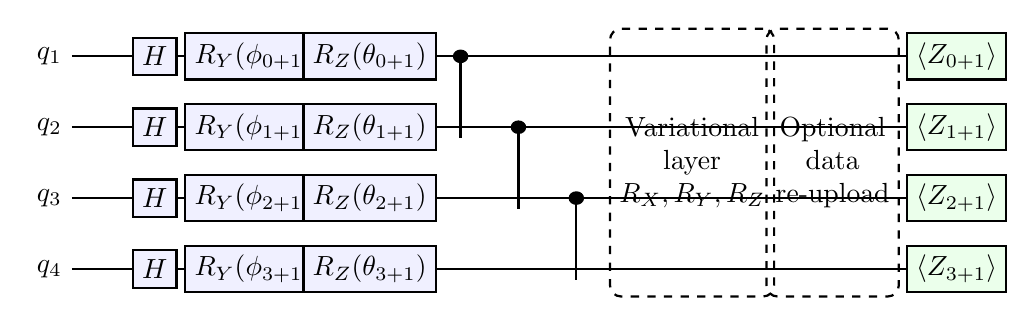
\begin{tikzpicture}[x=1.05cm,y=0.9cm, thick]
  \foreach \i/\label in {0/$q_1$,1/$q_2$,2/$q_3$,3/$q_4$} {
    \draw (0,-\i) -- (11.2,-\i);
    \node[left] at (0,-\i) {\label};
  }

  \foreach \i in {0,1,2,3} {
    \node[draw, minimum width=0.55cm, minimum height=0.45cm, fill=blue!6] at (1,-\i) {$H$};
    \node[draw, minimum width=0.9cm, minimum height=0.45cm, fill=blue!6] at (2.2,-\i) {$R_Y(\phi_{\i+1})$};
    \node[draw, minimum width=0.9cm, minimum height=0.45cm, fill=blue!6] at (3.6,-\i) {$R_Z(\theta_{\i+1})$};
  }

  \draw (4.7,0) circle (0.08);
  \fill (4.7,0) circle (0.08);
  \draw (4.7,0) -- (4.7,-1);
  \draw (4.55,-1) -- (4.85,-1);
  \draw (4.7,-1.15) -- (4.7,-0.85);

  \draw (5.4,-1) circle (0.08);
  \fill (5.4,-1) circle (0.08);
  \draw (5.4,-1) -- (5.4,-2);
  \draw (5.25,-2) -- (5.55,-2);
  \draw (5.4,-2.15) -- (5.4,-1.85);

  \draw (6.1,-2) circle (0.08);
  \fill (6.1,-2) circle (0.08);
  \draw (6.1,-2) -- (6.1,-3);
  \draw (5.95,-3) -- (6.25,-3);
  \draw (6.1,-3.15) -- (6.1,-2.85);

  \node[draw, dashed, rounded corners, minimum width=1.4cm, minimum height=3.4cm, align=center] at (7.5,-1.5) {Variational\\layer\\$R_X,R_Y,R_Z$};
  \node[draw, dashed, rounded corners, minimum width=1.2cm, minimum height=3.4cm, align=center] at (9.2,-1.5) {Optional\\data\\re-upload};

  \foreach \i in {0,1,2,3} {
    \node[draw, minimum width=1.1cm, minimum height=0.45cm, fill=green!8] at (10.7,-\i) {$\langle Z_{\i+1} \rangle$};
  }
\end{tikzpicture}
\caption{Schematic view of the quantum circuit inside the residual block for a 4-qubit configuration. The circuit consists of: Hadamard initialization, data-dependent angle embeddings ($R_Y$, $R_Z$), entangling CNOT gates in circular topology, trainable variational rotations ($R_X$, $R_Y$, $R_Z$), optional data re-uploading between layers, and Pauli-$Z$ expectation value measurements.}
\label{fig:quantum-layer}
\end{figure}


\subsection{Experimentation Pipeline}

This section describes the complete experimental setup, including data preparation, model configuration, training protocol, and evaluation methodology.

\subsubsection*{Data Preparation}

The raw input is a joined California wildfire--insurance--census--weather dataset at the ZIP-code--year level. The preprocessing script (\texttt{scripts/preprocess.py}) aggregates this into ZIP-year panels spanning 2018--2021. Two dataset variants are produced:

\begin{itemize}
  \item \textbf{Minimal dataset (9 features):} Contains the core wildfire risk, insurance, and weather variables needed for forecasting. This serves as a controlled baseline to evaluate model performance on a compact feature set.
  \item \textbf{Extended dataset (20 features):} Augments the minimal set with engineered variables including temperature range, drought proxy, log precipitation, dry-hot indicators, total burned acres, binary fire-occurrence signal, socioeconomic indices (total population, median income, poverty rate, education rate, vacancy rate, housing value, housing-cost burden, vulnerability index), and cyclical sine/cosine year encodings. This richer feature set provides more opportunity for cross-variable interaction and tests whether quantum-enhanced routing can exploit the additional information.
\end{itemize}

Only ZIP codes with complete 4-year panels (no missing values in any feature or target column) are retained. After filtering, the ZIP-code panels are shuffled with a fixed random seed and partitioned for model selection.

\subsubsection*{Panel Structure and Forecasting Formulation}

Each ZIP code produces one training sample consisting of:
\begin{itemize}
  \item \textbf{Encoder input} ($x_\text{enc}$): a tensor of shape $[3, F]$, where $F$ is the number of features (9 or 20), containing the feature values for years 2018, 2019, and 2020.
  \item \textbf{Decoder input} ($x_\text{dec}$): a tensor of shape $[4, F]$, constructed by concatenating the 3-step history with a zero-filled placeholder for the prediction step. This follows the standard TSLib encoder--decoder interface.
  \item \textbf{Target}: the \texttt{avg\_fire\_risk\_score} value for 2021.
  \item \textbf{Time marks}: month, day, day-of-week, and hour encodings derived from January 1st of each year, following TSLib's time-mark convention.
\end{itemize}

The task is therefore a multivariate-input, univariate-output forecasting problem: the model consumes 3 annual time steps of $F$ features and predicts 1 future time step of the target variable.

\subsubsection*{Data Normalization}

A \texttt{StandardScaler} (zero mean, unit variance) is fitted \emph{exclusively} on the training partition's feature and target values. The same scaler is then applied to the validation and test partitions without refitting, preventing information leakage. All model training and evaluation operate on the normalized data. Final metric computation inverts the normalization on both predictions and ground truth before computing error statistics in the original scale.

\subsubsection*{Split Modes}

Two evaluation protocols are supported:

\begin{enumerate}
  \item \textbf{Full-2021 mode (default).} ZIP-code panels are split into a training set (85\%) and a validation set (15\%) for model selection. After identifying the best epoch via early stopping on the validation loss, the model is \emph{refit from scratch} on all ZIP panels for the same number of epochs, and predictions are emitted for the entire 2021 panel. This deployment-style protocol maximizes the data available for the final model and produces predictions for all ZIP codes.

  \item \textbf{ZIP-holdout mode (legacy benchmark).} ZIP-code panels are split into training (70\%), validation (15\%), and test (15\%) partitions. The model is trained with early stopping on the validation loss, and final metrics are computed on the held-out test ZIP codes. This protocol provides a standard held-out evaluation but produces predictions only for the test partition.
\end{enumerate}

\subsubsection*{Training Protocol}

All models---classical and quantum-enhanced---are trained using the same protocol to ensure fair comparison:

\begin{itemize}
  \item \textbf{Optimizer:} Adam with default momentum parameters ($\beta_1 = 0.9$, $\beta_2 = 0.999$).
  \item \textbf{Learning rate:} $10^{-3}$ (fixed; no learning rate scheduling is applied during the retained experiments).
  \item \textbf{Weight decay:} $0$ (no $L_2$ regularization).
  \item \textbf{Loss function:} Mean squared error (MSE) computed on the normalized target values.
  \item \textbf{Maximum epochs:} 50.
  \item \textbf{Early stopping:} Patience of 10 epochs. If the validation MSE does not improve for 10 consecutive epochs, training halts and the model state from the best validation epoch is restored. This prevents overfitting and reduces unnecessary computation, particularly for quantum models where each epoch involves VQC forward and backward passes.
  \item \textbf{Batch size:} 128 ZIP-code samples per mini-batch. Given the dataset size (hundreds of complete ZIP panels), this typically results in a small number of gradient steps per epoch.
  \item \textbf{Random seed:} 42, applied to Python's \texttt{random}, NumPy, and PyTorch (CPU and CUDA) random number generators. The seed controls data shuffling, parameter initialization, and DataLoader ordering, ensuring reproducibility across runs.
  \item \textbf{Gradient computation for quantum layers:} PennyLane's parameter-shift rule or backpropagation mode (depending on the backend) computes gradients through the quantum circuit. The \texttt{default.qubit} backend supports analytic backpropagation, which is exact and avoids the statistical noise of shot-based gradient estimation.
\end{itemize}

\subsubsection*{Classical Backbone Hyperparameters}

All classical and hybrid models share the same backbone configuration to isolate the effect of quantum enhancement:

\begin{center}
\begin{tabular}{ll}
\toprule
Parameter & Value \\
\midrule
Model dimension ($d_\text{model}$) & 32 \\
Feedforward dimension ($d_\text{ff}$) & 64 \\
Encoder layers ($e_\text{layers}$) & 2 \\
Decoder layers ($d_\text{layers}$) & 1 \\
Attention heads ($n_\text{heads}$) & 4 \\
Dropout & 0.1 \\
Activation & GELU \\
Input sequence length & 3 \\
Prediction length & 1 \\
\bottomrule
\end{tabular}
\end{center}

For FreTS-based models, the embedding dimension is 128 and the prediction head hidden size is 256, following the original FreTS implementation. For Crossformer-based models, the segment length is 12 and the window merging size is 2.

\subsubsection*{Quantum Hyperparameters}

The quantum configuration for the retained experiments:

\begin{center}
\begin{tabular}{ll}
\toprule
Parameter & Value \\
\midrule
Number of qubits ($n_q$) & 4 \\
Variational layers ($L$) & 1 or 2 \\
Entangling steps ($n_e$) & 1 \\
Data re-uploading & Enabled (in best runs) \\
Quantum backend & \texttt{default.qubit} (PennyLane statevector simulator) \\
Trainable quantum parameters per block & $3 \times n_q \times L$ (12 or 24) \\
\bottomrule
\end{tabular}
\end{center}

With 4 qubits, 1 variational layer, and 1 entangling step, each quantum residual block adds only 12 trainable parameters beyond the classical projection weights. This is intentionally compact: the quantum circuit is meant to contribute structured nonlinearity through entanglement, not additional parameter capacity.

\subsubsection*{Evaluation Metrics}

Performance is evaluated using four standard regression metrics, all computed on the original (un-normalized) scale:

\begin{itemize}
  \item \textbf{MAE} (Mean Absolute Error): $\frac{1}{n}\sum_{i=1}^{n}|y_i - \hat{y}_i|$
  \item \textbf{MSE} (Mean Squared Error): $\frac{1}{n}\sum_{i=1}^{n}(y_i - \hat{y}_i)^2$
  \item \textbf{RMSE} (Root Mean Squared Error): $\sqrt{\text{MSE}}$
  \item \textbf{$R^2$} (Coefficient of Determination): $1 - \frac{\sum_{i=1}^{n}(y_i - \hat{y}_i)^2}{\sum_{i=1}^{n}(y_i - \bar{y})^2}$
\end{itemize}

where $y_i$ is the true value, $\hat{y}_i$ is the predicted value, and $\bar{y}$ is the mean of the true values over the evaluation set.

\subsubsection*{Benchmark Scope}

The full benchmark evaluates 25+ classical models from the Time-Series-Library alongside the two deep quantum variants and their shallow quantum wrapper counterparts. Models that are architecturally incompatible with the 3-step panel format (e.g., those requiring longer input sequences, hardcoded patch sizes, or specialized data loaders) are automatically detected during a preflight compatibility check and excluded with documented reasons. Each model--dataset combination is trained and evaluated independently, and all results, training histories, and per-ZIP predictions are archived in a structured experiment directory with a unique run tag.

\subsection{Underlying Assumptions}

The method relies on the following assumptions:
\begin{itemize}
  \item Complete four-year ZIP panels are representative enough to build a stable forecasting benchmark, despite the limited temporal depth.
  \item Wildfire risk and insurance premiums can benefit from cross-variable interactions that are not purely linear, justifying the use of entanglement-based nonlinear mixing.
  \item A low-qubit VQC can act as a useful nonlinear bottleneck even when the full sequence model remains classical, because the bottleneck operates on already-compressed representations.
  \item Simulator-based results on \texttt{default.qubit} are an acceptable proxy for the resource profile of a near-term quantum workflow, given that the circuits are shallow (1--2 layers) and narrow (4 qubits).
\end{itemize}

\subsection{Additional Data Used}

No external third-party data were added beyond the provided joined wildfire--insurance--census--weather dataset. However, the solution uses additional engineered variables derived from the provided fields, including:
\begin{itemize}
  \item weather-derived features: temperature range ($T_\text{max} - T_\text{min}$), drought proxy, log-transformed precipitation, and dry-hot indicator variables;
  \item wildfire-derived features: total burned acres (sum of \texttt{GIS\_ACRES}) and a binary fire-occurrence signal;
  \item socioeconomic variables: total population, median income, poverty rate, education rate, vacancy rate, housing value, housing-cost burden, and a composite vulnerability index;
  \item insurance-derived variables (for Task~2): rolling premium mean, loss ratio, claim frequency, average loss per claim, and year-over-year premium growth;
  \item temporal encodings: cyclical sine and cosine transforms of the year index.
\end{itemize}

\subsection{Evaluation}

The evaluation protocol compares deep quantum variants against the full suite of retained classical time-series baselines from the same library. The purpose is twofold: (i) to assess whether quantum layers can improve interaction-heavy architectural stages without destabilizing training, and (ii) to determine the conditions (feature richness, qubit count, circuit depth) under which quantum enhancement is most effective.

The most relevant comparison points supported by the retained experiments are:
\begin{itemize}
  \item classical \texttt{FreTS} vs.\ \texttt{QFreTS\_Deep} on the minimal and extended datasets;
  \item classical \texttt{Crossformer} vs.\ \texttt{QCrossformer\_Deep} on the minimal and extended datasets;
  \item ablations over qubit count (2, 4, 6), variational depth (1, 2, 3), and data re-uploading (on/off).
\end{itemize}


\section{Description of Results and Repository}

[Results tables to be inserted here.]

The repository containing the code used to run the algorithm is:
\[
\href{https://github.com/tawheedrony/deloitte_challenge_2025}{https://github.com/tawheedrony/deloitte\_challenge\_2025}
\]


\section{Description of the Envisioned Algorithm}

The envisioned full solution is a chained two-stage system:
\begin{enumerate}
  \item Predict wildfire risk for each ZIP code using the hybrid quantum Task~1A model.
  \item Inject the predicted 2021 risk score into the insurance dataset as a new explanatory feature.
  \item Train a second forecasting model for insurance premiums using both the historical insurance trajectory and the upstream wildfire-risk forecast.
\end{enumerate}

The expected benefits are:
\begin{itemize}
  \item Tighter coupling between physical hazard forecasts and economic risk estimates, so that changes in wildfire exposure are reflected in premium predictions.
  \item Better predictive performance for premiums in areas where wildfire exposure materially changes insurer behavior, since the insurance model can condition on a forward-looking risk estimate rather than a lagged historical proxy.
  \item Improved interpretability because the insurance model explicitly conditions on a forecast wildfire-risk score, making it possible to trace how changes in predicted fire risk propagate to predicted premium changes.
\end{itemize}

The main practical requirements for the full solution are:
\begin{itemize}
  \item Complete and temporally aligned ZIP-level wildfire, insurance, weather, and census panels covering both the training history and the target year.
  \item A reproducible Task~1A prediction pipeline with archived run configurations, so that the exact wildfire-risk predictions used as Task~2 inputs can be traced back to a specific model checkpoint and hyperparameter setting.
  \item Calibrated uncertainty estimates so downstream insurance forecasts can account for error propagation from the Task~1A stage.
  \item Hardware-aware quantum circuit design, since real-device deployment would require low circuit depth, limited qubit count, and noise-robust gate sequences compatible with the connectivity constraints of near-term quantum processors.
\end{itemize}

\section{Other Aspects}

\subsection*{Resource Requirements}

The retained quantum experiments were executed on the PennyLane \texttt{default.qubit} statevector simulator using compact VQCs with 4 qubits, 1--2 variational layers, and 1 entangling step. This choice keeps the quantum portion shallow and consistent with near-term hardware constraints. All experiments were run on commodity CPU hardware without GPU acceleration for the quantum simulation. The classical backbone computations (attention, FFT, linear layers) can optionally use GPU acceleration when available.

\subsection*{Reproducibility}

The repository stores preprocessing scripts, model definitions, benchmark scripts, run manifests (JSON configuration files recording all hyperparameters and split settings), per-ZIP prediction CSV files, and per-epoch training histories. Each experiment run is tagged with a unique identifier and stored in an immutable directory structure. This allows any reported result to be reproduced by re-running the benchmark script with the corresponding run configuration and random seed.

\subsection*{Limitations}

The current repository benchmark is narrower than the original challenge description because it uses complete 2018--2021 panels rather than full 2018--2022 histories with a 2023 target. Therefore, the reported results should be interpreted as a reproducible proxy benchmark on available data and not as a final claim on the original target year. Additionally, the quantum circuits are evaluated on a statevector simulator, which does not account for hardware noise, limited connectivity, or finite shot counts that would affect performance on real quantum processors.

\end{document}
